\chapter{A Primeira Lei da termodinâmica}
\label{chap:theFirstLaw}

    Consideremos o sistema fechado entre os estados infinitesimais 1 e 2. Vamos
    repetir aqui a figura 0.2 com a representação em forma de grafo de vários
    processos entre os mesmos estados.

    \begin{figure}[!htb]
        \caption{%
            Representação em forma de grafo dos processos em um sistema.
        }

        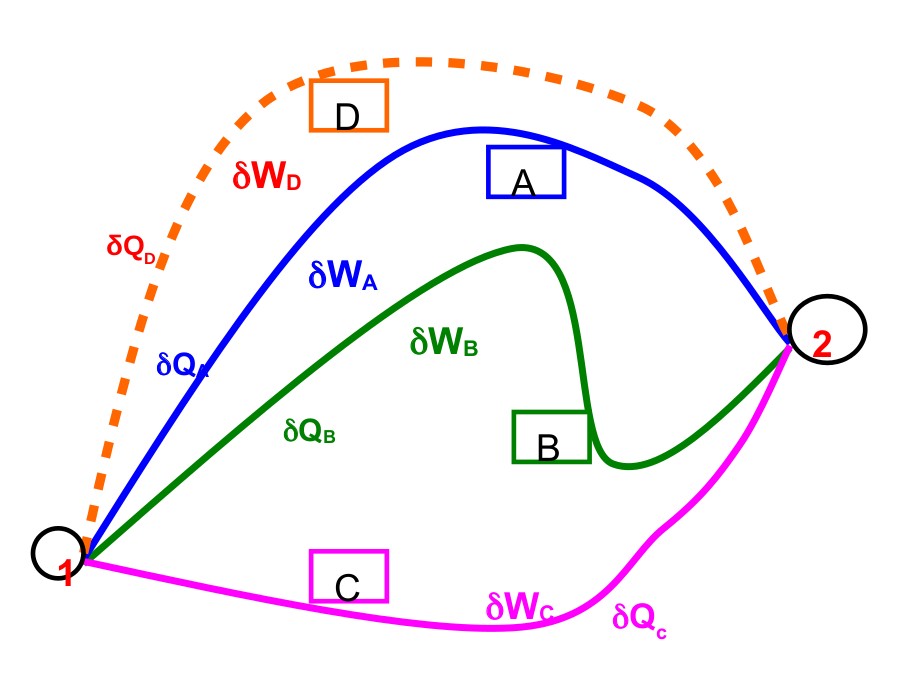
\includegraphics[
            width=0.45\textwidth
        ]   {thermodynamicProcesses.tex}

        \label{fig:thermodynamicProcessesFirstLawChapter}
    \end{figure}

    Sejam os processos infinitesimais A, B, C reversíveis e D irreversível
    entre os estados 1 e 2 (o que é mesmo um processo reversível?). Sabemos
    que, de um modo geral, %
    \idiff{\gls{heatTransfer}_{A}} $\neq$ %
    \idiff{\gls{heatTransfer}_{B}} $\neq$ %
    \idiff{\gls{heatTransfer}_{C}} $\neq$ %
    \idiff{\gls{heatTransfer}_{D}} e %
    \idiff{\gls{workTransfer}_{A}} $\neq$ %
    \idiff{\gls{workTransfer}_{B}} $\neq$ %
    \idiff{\gls{workTransfer}_{C}} $\neq$ %
    \idiff{\gls{workTransfer}_{D}}, %
    ou seja, o calor e o trabalho associados a cada processo são diferentes
    para cada processo.

    Entretanto, observa-se que, para qualquer processo que leva do estado 1
    para o estado 2 do sistema fechado da
    \cref{fig:thermodynamicProcessesFirstLawChapter}:
    %
    \begin{equation} \label{eq:2.1}
        \idiff{\gls{heatTransfer}_{A}} - \idiff{\gls{workTransfer}_{A}}
        =
        \idiff{\gls{heatTransfer}_{B}} - \idiff{\gls{workTransfer}_{B}}
        =
        \idiff{\gls{heatTransfer}_{C}} - \idiff{\gls{workTransfer}_{C}}
        =
        \idiff{\gls{heatTransfer}_{D}} - \idiff{\gls{workTransfer}_{D}}
        =
        \idiff{\gls{heatTransfer}} - \idiff{\gls{workTransfer}}\,.
    \end{equation}

    Note que esta diferença se mantém constante não importando o processo que
    escolhermos entre 1 e 2. Sendo assim, podemos atribuir a ela o caráter de
    uma variação de uma propriedade termodinâmica no interior do sistema.
    Vamos chamá-la de variação da energia total do sistema
    \diff{\gls{totalEnergy}}. Então
	%
	\begin{equation} \label{eq:2.2}
        \diff{\gls{totalEnergy}}
        \defeq
        \idiff{\gls{heatTransfer}}
        -
        \idiff{\gls{workTransfer}}
    \end{equation}
    %
    ou, integrando-se a \cref{eq:2.2} para variações finitas de estado,
    %
    \begin{subequations} \label{eq:2.3}
    \begin{equation}
        \fprocess{heatTransfer}{1}{2}{}
        -
        \fprocess{workTransfer}{1}{2}{}
        =
        \Delta \gls{totalEnergy}
        =
        \state{\gls{totalEnergy}}{2}
        -
        \state{\gls{totalEnergy}}{1}
    \end{equation}
    %
    \mbox{%
        \parbox{\textwidth}{%
            Na forma de diferenciais ou de equação diferencial, quando existem
            $j$ interações de calor na fronteira do sistema durante o processo:
        }
    }
    %
    \begin{equation}
        \underset{j}{\sum }{%
            \idiff{\gls{heatTransfer}}_j
        }
        -
        \idiff{\gls{workTransfer}}
        =
        \diff{\gls{totalEnergy}}
    \,\,\,\,
    %
    \text{ou}
    %
    \,\,\,\,
        \underset{j}{\sum }{%
            \transferRate{heatTransfer}_j
        }
        -
        \transferRate{workTransfer}
        =
        \DDt{\gls{totalEnergy}}\,.
    \end{equation}
    \end{subequations}

    As \cref{eq:2.2,eq:2.3} representam uma formulação matemática da Primeira
    Lei da Termodinâmica, ou da Conservação da Energia, e valem para todos os
    processos que ocorrerem em qualquer sistema fechado. Pode explicar porque é
    denominada Lei da Conservação de Energia?


    \section{Consequências da Primeira Lei para Sistema Fechado}

    Um processo é dito cíclico quando o estado inicial coincidir com o estado
    final do sistema ao término do processo. Ora, se o estado do sistema é
    definido pelo valor de suas propriedades, a estados idênticos correspondem
    idênticos valores para todas as propriedades do sistema, ou seja, em um
    processo cíclico, a variação de qualquer propriedade do sistema é zero para
    ciclos completos. Isto vale para \gls{temperature}, \gls{pressure},
    \gls{volume} e certamente também para a energia total \gls{totalEnergy},
    recém-definida. Em consequência desse fato,
    %
    \begin{equation}
        \Delta{\gls{totalEnergy}}
        =
        0
    \end{equation}
    %
    e portanto
    %
    \begin{equation} \label{eq:2.4}
        \underset{j}{\sum }{
            \oint{
                \idiff{\gls{heatTransfer}}_j
            }
        }
        =
        \oint{%
            \idiff{\gls{workTransfer}}
        }\,.
    \end{equation}

    O significado físico é que para qualquer processo cíclico que ocorra em
    sistema fechado, o trabalho total realizado pelo sistema é sempre
    exatamente igual ao calor total por ele recebido (ou, invertendo os sinais,
    o trabalho total efetuado sobre o sistema é exatamente igual ao calor total
    por ele dissipado).

    A \cref{eq:2.4} é muito importante e de fato muitos autores a escolhem como
    a definição da Primeira Lei da Termodinâmica. Nesse caso, a \cref{eq:2.2}
    deve ser por eles deduzida.

    Estamos interessados em produzir potência. Então, poderíamos selecionar um
    sistema fechado operando ciclicamente, e o utilizaríamos para bombear
    potência térmica de um reservatório de calor, obtendo assim potência
    mecânica indefinidamente. Aplicamos a Primeira Lei ao nosso sistema em um
    processo cíclico e concluiríamos que o trabalho mecânico obtido a cada
    ciclo seria igual ao calor retirado do reservatório térmico. Entretanto,
    logo descobriríamos que, embora sem violar a Primeira Lei, o nosso aparato
    jamais funcionaria!

    Imaginemos então que chegamos à conclusão que para funcionar, parte do
    calor recebido do reservatório térmico teria que ser rejeitada à
    vizinhança do sistema. É claro que quanto menor este calor rejeitado, maior
    a parcela do calor do reservatório térmico que se converte em trabalho
    mecânico. Então, a próxima pergunta seria: como obtermos o valor do menor
    calor que deve ser rejeitado para que o nosso aparato funcione? Observe que
    a resposta a esta questão, como veremos, não pode ser obtida com base
    puramente na Primeira Lei da Termodinâmica e terá que ser adiada até a
    discussão sobre a Segunda Lei. Convença-se então que a Primeira Lei da
    Termodinâmica é condição necessária para o funcionamento dos sistemas, mas
    não é suficiente.

    Agora, dentre todos os possíveis processos que conectam os mesmos dois
    estados de um sistema fechado, selecionemos um deles que seja adiabático.
    Então, pela primeira lei:
    %
    \begin{equation} \label{eq:2.5}
        \idiff{\gls{workTransfer}}
        =
        \diff{\gls{totalEnergy}}\,,
        \,\,\,\,
        \text{pois \idiff{\gls{heatTransfer}} $= 0$ (processo adiabático)}
    \end{equation}
    %
    e, uma vez que \diff{\gls{totalEnergy}} não depende de nenhum processo,
    concluímos que o trabalho realizado por qualquer processo adiabático que
    conecte os mesmos estados de um sistema fechado é independente do processo.
    Este é o princípio da conservação da energia mecânica. Por um raciocínio
    análogo, o calor envolvido nos processos de zero-trabalho entre os mesmos
    estados de um sistema fechado também é independente do processo e este
    seria o princípio da conservação da energia térmica.

    Além disso, se o processo for adiabático e de zero-trabalho ao mesmo tempo
    (lembra-se? um sistema isolado) o que acontecerá com a variação da energia
    total? Isso mesmo, a energia total de um sistema isolado não se alterará
    jamais! Percebe de onde vem a noção de conservação de energia? Atenção:
    aqui não se trata de processo cíclico --- todas as demais propriedades
    termodinâmicas podem se alterar, exceto a energia total do sistema.


    \section{Energia Interna, Cinética e Potencial}

    Do que se trata, afinal de contas, esta tal de energia total? Considere um
    volume de gás de massa \gls{mass} e temperatura \gls{temperature} encerrado
    em um recipiente rígido e adiabático.  Admita que o recipiente com o gás
    esteja em movimento com uma velocidade \gls{velocity}, em uma cota vertical
    \gls{zAxis}. Sabemos que, nessas condições, o gás possui suas energias
    cinética \gls{kineticEnergy} e potencial \gls{potentialEnergy}  dadas
    respectivamente pelas expressões
    %
    \begin{equation} \label{eq:2.6}
        \gls{kineticEnergy}
        =
        \frac{\gls{mass}}{2}
        \gls{velocityComp}^2
        %
        \,\,\,\,
        \text{e}
        \,\,\,\,
        %
        \gls{potentialEnergy}
        =
        \gls{mass}
        \gls{gravityComp}
        \gls{zAxis}\,.
    \end{equation}

    Sabemos que a energia total \gls{totalEnergy} deste gás (desprezando-se o
    recipiente), que está isolado, não deve se alterar.  Se a energia total
    fosse apenas a soma da sua energia cinética com a energia potencial, como
    poderia \gls{totalEnergy} manter-se inalterado, se a velocidade
    \gls{velocity} e a cota \gls{zAxis} podem ser facilmente modificadas?  Ora,
    então, se subtrairmos a soma das energias cinética e potencial da energia
    total do sistema, o que resta deve ser também uma forma de energia.  Por
    outro lado, as moléculas dentro do gás estão em um agitado movimento que,
    de acordo com a teoria cinética dos gases, depende da sua temperatura
    \gls{temperature}. Concluímos que esta agitação térmica das moléculas tem a
    sua representação macroscópica expressa através desta nova forma de
    energia, a energia interna \gls{internalEnergy}. Assim,
    %
    \begin{equation} \label{eq:2.7}
        \gls{totalEnergy}
        =
        \gls{internalEnergy}
        +
        \gls{kineticEnergy}
        +
        \gls{potentialEnergy}\,.
    \end{equation}

    Se admitirmos (hipótese que adotaremos muitas vezes) que que
    $\gls{kineticEnergy} = \gls{potentialEnergy} = 0$ então $\gls{totalEnergy}
    = \gls{internalEnergy}$. Note que dividindo-se a energia interna do sistema
    \gls{internalEnergy} pela sua massa \gls{mass}, obteremos a energia interna
    específica \gls{intInternalEnergy} e pelo número de moles
    \gls{numberMoles}, a energia interna específica molar
    \molar{\gls{intInternalEnergy}}.

    Pois bem, sabemos que a agitação térmica das moléculas do nosso gás e,
    portanto, a sua energia interna, depende, graças à teoria cinética dos
    gases, da temperatura do gás. O que poderíamos dizer a respeito da energia
    interna dos líquidos? Imagine a água líquida e o seu vapor à pressão
    ambiente: você pode dizer qual seria a fase cuja energia interna seria
    maior?

    A conservação da energia interna de um sistema isolado é muito útil.
    Vejamos o exemplo clássico da mistura de gases a partir de uma expansão não
    resistida, representado na \cref{fig:nonResistedExpansion}. Seja um gás em
    estados distintos $A$ e $B$ em cada uma das partições de um recipiente
    rígido e adiabático de volume \gls{volume}, tal que cada um ocupa uma
    fração do volume total e separados apenas por uma membrana também rígida e
    adiabática. Rompe-se então a membrana e as porções do gás nas partições se
    misturam. Quanto vale então a energia interna da mistura final do gás?

    \begin{figure}[!htb]
        \caption{%
            Exemplo de expansão não-resistida.
        }

        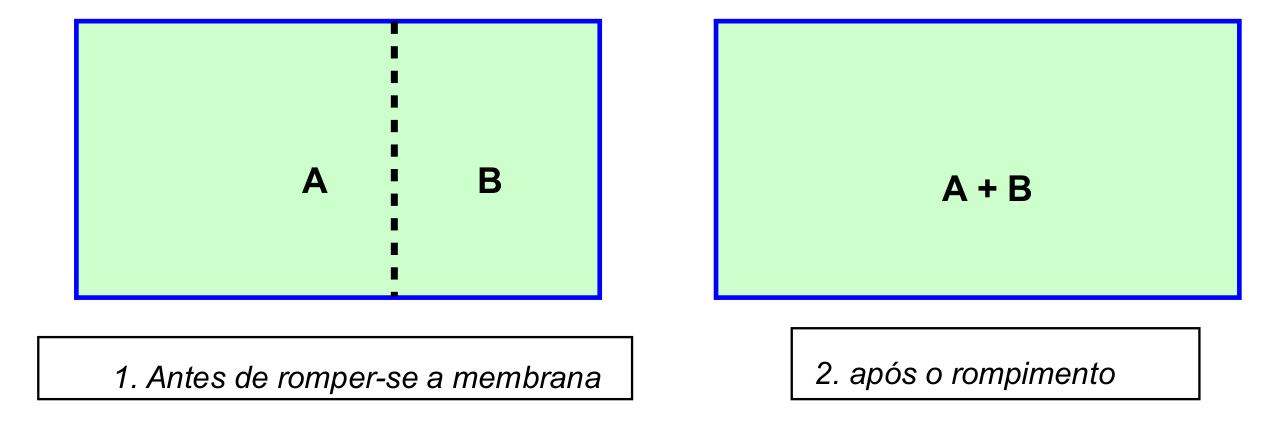
\includegraphics[
            width=0.75\textwidth
        ]   {nonResistedExpansion.tex}

        \label{fig:nonResistedExpansion}
    \end{figure}

    Vamos desprezar as energias cinética e potencial. Podemos descrever o
    processo como evoluindo de um estado 1 para um estado 2, como será
    descrito.

    \begin{itemize}
        \item Estado 1:

            De acordo com a nossa definição de sistema, poderemos escolher como
            o sistema o volume encerrado pelo gás nos estados A e B. Este é
            claramente composto de dois subsistemas: o gás com energia interna
            $\state{\gls{internalEnergy}}{1}_{A}$ e massa
            $\state{\gls{mass}}{1}_{A}$  e o gás com energia interna
            $\state{\gls{internalEnergy}}{1}_{B}$ e massa
            $\state{\gls{mass}}{1}_{B}$.

            A energia interna do sistema neste estado é a soma das energias
            internas dos seus subsistemas. A propósito, este princípio vale
            para qualquer propriedade extensiva.

            Por exemplo, o volume \state{\gls{volume}}{1} do sistema é a soma
            $\state{\gls{volume}}{1}_{A} + \state{\gls{volume}}{1}_{B}$.
            Entretanto, assuma como um princípio fundamental que nunca se podem
            somar propriedades intensivas entre si, ou seja, não se pode
            escrever-se $\state{\gls{specificVolume}}{1} +
            \state{\gls{specificVolume}}{1}$ ou $\state{\gls{temperature}}{1} +
            \state{\gls{temperature}}{2}$.

            No estado 1 não tem sentido falarem-se em temperatura e pressão do
            sistema pois os dois subsistemas podem estar a temperaturas
            $\state{\gls{temperature}}{1}_{A},\state{\gls{pressure}}{1}_{A}$ e
            $\state{\gls{temperature}}{1}_{B},\state{\gls{pressure}}{1}_{B}$
            completamente diferentes (você pode dizer por quê?).

        \item Estado 2:

            O sistema gás torna-se uma mistura homogênea, cuja definição mais
            formal será vista mais tarde. Como escolhemos um sistema fechado, a
            massa do sistema \state{\gls{mass}}{2} permanece sendo
            $\state{\gls{mass}}{1}_{A}$ + $\state{\gls{mass}}{1}_{B}$. A
            energia interna agora provém da mistura do gás em A e em B
            originalmente no estado 1.

    \end{itemize}

    Então, quanto vale a energia interna do sistema no estado 1?
	%
	\begin{equation} \label{eq:2.8}
        \state{\gls{internalEnergy}}{1}
        =
        \state{\gls{internalEnergy}}{1}_{A}
        +
        \state{\gls{internalEnergy}}{1}_{B}
        =
        \state{\gls{mass}}{1}_{A}
        \state{\gls{intInternalEnergy}}{1}_{A}
        \functionOf{
            \state{\gls{temperature}}{1}_{A},
            \state{\gls{pressure}}{1}_{A}
        }
        +
        \state{\gls{mass}}{1}_{B}
        \state{\gls{intInternalEnergy}}{1}_{B}
        \functionOf{
            \state{\gls{temperature}}{1}_{B},
            \state{\gls{pressure}}{1}_{B}
        }\,.
    \end{equation}

    Quanto vale a energia interna do sistema no estado 2?
    %
    \begin{equation} \label{eq:2.9}
        \state{\gls{internalEnergy}}{2}
        =
        m^{(2)}
        \state{\gls{intInternalEnergy}}{2}
        =
        \left(
            \state{\gls{mass}}{1}_{A}
            +
            \state{\gls{mass}}{1}_{B}
        \right)
        \state{\gls{intInternalEnergy}}{2}
        \functionOf{
            \state{\gls{temperature}}{2},
            \state{\gls{pressure}}{2}
        }\,.
    \end{equation}

    Aplicando-se a Primeira Lei, obtém-se que $\state{\gls{internalEnergy}}{1} =
    \state{\gls{internalEnergy}}{2}$ e assim podemos escrever que
    %
    \begin{equation} \label{eq:2.10}
        \left(
            \state{\gls{mass}}{1}_{A}
            +
            \state{\gls{mass}}{1}_{B}
        \right)
        \state{\gls{intInternalEnergy}}{2}
        \functionOf{
            \state{\gls{temperature}}{2},
            \state{\gls{pressure}}{2}
        }
        =
        \state{\gls{mass}}{1}_{A}
        \state{\gls{intInternalEnergy}}{1}_{A}
        \functionOf{
            \state{\gls{temperature}}{1}_{A},
            \state{\gls{pressure}}{1}_{A}
        }
        +
        \state{\gls{mass}}{1}_{B}
        \state{\gls{intInternalEnergy}}{1}_{B}
        \functionOf{
            \state{\gls{temperature}}{1}_{B},
            \state{\gls{pressure}}{1}_{B}
        }\,.
    \end{equation}

    Portanto, para este sistema e presente processo, a energia interna
    específica do gás nos estado 2 após o rompimento da membrana é dada pela
    média, ponderada pelas massas, das energias internas específicas do gás nos
    estados A e B, calculadas antes do rompimento da membrana, estado 1.

    Podemos rearranjar também da seguinte forma:
    %
    \begin{equation} \label{eq:2.11}
        \state{\gls{mass}}{1}_{A}
        \left[
            \state{\gls{intInternalEnergy}}{2}
            \functionOf{
                \state{\gls{temperature}}{2},
                \state{\gls{pressure}}{2}
            }
            -
            \state{\gls{intInternalEnergy}}{1}_{A}
            \functionOf{
                \state{\gls{temperature}}{1}_{A},
                \state{\gls{pressure}}{1}_{A}
            }
        \right]
        +
        \state{\gls{mass}}{1}_{B}
        \left[
            \state{\gls{intInternalEnergy}}{2}
            \functionOf{
                \state{\gls{temperature}}{2},
                \state{\gls{pressure}}{2}
            }
            -
            \state{\gls{intInternalEnergy}}{1}_{B}
            \functionOf{
                \state{\gls{temperature}}{1}_{B},
                \state{\gls{pressure}}{1}_{B}
            }
        \right]
        =
        0\,.
    \end{equation}

    A \cref{eq:2.11} ilustra o seguinte princípio, que se aplica a todas as
    equações termodinâmicas: é sempre possível restruturarem-se as equações na
    forma de diferenças de propriedades termodinâmicas, embora às vezes isto
    não seja fácil ou aparente.

    Concluímos, também, como uma consequência das Leis, que o valor de uma
    propriedade termodinâmica referente a um estado é arbitrário, ou seja,
    depende de uma base arbitrariamente escolhida.

    Além disso, para manter a consistência física das equações, as diferenças
    das propriedades termodinâmicas não podem depender das bases estabelecidas
    para sua determinação. Este resultado é extremamente importante e será
    utilizado inúmeras vezes em nosso estudo.

    Como poderíamos determinar a temperatura e pressão finais
    \state{\gls{temperature}}{2} e \state{\gls{pressure}}{2} da mistura resultante? Você
    deve se convencer que na \cref{eq:2.10} (ou \ref{eq:2.11}) as únicas
    incógnitas são \state{\gls{temperature}}{2} e \state{\gls{pressure}}{2}.  Entretanto,
    temos apenas uma equação. Para fechar o sistema precisamos de mais uma
    equação. Sabe dizer qual é?


    \section{O Sistema Aberto ou Volume de Controle}

    Até este ponto de nosso estudo não havíamos permitido as interações de
    massa através da fronteira do sistema. Entretanto, nem sempre conseguiremos
    modelar os nossos problemas reais por meio de sistemas fechados.  Relaxando
    então esta restrição, ou seja, permitindo o transporte de massa através de
    qualquer parte da fronteira, obtemos um sistema aberto, ou volume de
    controle. Para o volume de controle, a fronteira costuma ser denominada
    também de superfície de controle. Em relação ao sistema aberto da
    \cref{fig:nonResistedExpansion}, sejam os calores
    $\idiff{\gls{heatTransfer}}_j$ provenientes dos reservatórios de calor a
    \state{\gls{temperature}}{j}, o calor
    \idiff{\gsub{heatTransfer}{environmentState}} proveniente do reservatório do
    meio-ambiente a \gsub{temperature}{environmentState}, o trabalho mecânico
    \idiff{\gsub{workTransfer}{controlVolume}} e as massas que entram no
    sistema $\idiff{\gls{mass}_{\gsub{inlet}{k}}}$ e que saem do sistema, tudo
    durante o intervalo \diff{\gls{time}}. Note que na repressentação separamos
    o calor proveniente do reservatório do meio-ambiente por conveniência
    futura. Nesse mesmo intervalo de tempo, as interações na fronteira causarão
    no interior do sistema a alteração de muitas de suas propriedades
    termodinâmicas, dentre as quais já conhecemos pelo menos
    \diff{\gsub{temperature}{controlVolume}},
    \diff{\gsub{volume}{controlVolume}},
    \diff{\gsub{specificVolume}{controlVolume}},
    \diff{\gsub{pressure}{controlVolume}}, \diff{\gsub{mass}{controlVolume}},
    \diff{\gsub{totalEnergy}{controlVolume}},
    \diff{\gls{intTotalEnergy}{controlVOlume}},
    \diff{\gsub{internalEnergy}{controlVolume}},
    \diff{\gsub{intInternalEnergy}{controlVolume}}.  Você é capaz de
    identificar cada uma delas? Verifique que para a energia total no volume de
    controle:
    %
    \begin{equation}
        \diff{\gsub{totalEnergy}{controlVolume}}
        =
        \diff{
            \gsub{mass}{controlVolume}
            \gsub{intTotalEnergy}{controlVolume}
        }
        =
        \gsub{mass}{controlVolume}
        \diff{
            \gsub{intTotalEnergy}{controlVolume}
        }
        +
        \gsub{intTotalEnergy}{controlVolume}
        \diff{
            \gsub{mass}{controlVolume}
        }\,,
    \end{equation}
    %
    e uma expressão análoga pode ser obtida para qualquer propriedade extensiva
    relativamente a sua respectiva propriedade intensivada e a massa.


    \section{A Conservação da Massa para Sistema Aberto}

    Sabemos que, fora do contexto relativístico, massa não pode ser destruída e
    nem produzida. Sendo assim, deveremos ser capazes de, uma vez identificado
    o sistema, manter durante qualquer intervalo de tempo \diff{\gls{time}} um
    preciso inventário da massa que entra e que sai através da superfície de
    controle, bem como daquela que permanece dentro do \gls{vc}. Para sistemas
    fechados, a conservação da massa é trivialmente satisfeita. O que devemos
    sempre lembrar no momento da escolha do sistema fechado, é que a massa em
    seu interior tem que se manter invariante a qualquer custo.

    A conservação de massa para o sistema aberto pode matematicamente ser
    expressa como:
    %
    \begin{equation} \label{eq:2.12}
        \diff{\gsub{mass}{controlVolume}}
        =
        \underset{\gls{inlet}}{\sum }{
            \idiff{\gsub{mass}{inlet}}
        }
        -
        \underset{\gls{outlet}}{\sum }{
            \idiff{\gsub{mass}{outlet}}
        }
    \end{equation}
    %
    ou
    %
    \begin{equation} \label{eq:2.13}
        \DDt{\gsub{mass}{controlVolume}}
        =
        \underset{\gls{inlet}}{\sum }{
            \transferRate{mass}_{\gls{inlet}}
        }
        -
        \underset{\gls{outlet}}{\sum }{
            \transferRate{mass}_{\gls{outlet}}
        }
    \end{equation}
    %
    onde $\underset{\gls{inlet}}{\sum }{\transferRate{mass}_{\gls{inlet}}}$  é
    a soma das vazões de massas que entram no \gls{vc} e
    $\underset{\gls{outlet}}{\sum }{\transferRate{mass}_{\gls{outlet}}}$ é a
    soma das vazões de massas que saem do VC no intervalo de tempo dt e a
    somatória se aplica a todas as entradas e saídas de massa na superfície de
    controle.


    \section{A Primeira Lei para Volume de Controle}

    Vimos, pela Primeira Lei para sistema fechado, que a diferença entre as
    interações de calor e de trabalho não depende do processo e denominamos
    esta diferença de variação da energia total do sistema, que é a soma da
    variação de sua energia cinética, potencial e interna. De fato, estamos
    procedendo a um inventário de energia no sistema. Em um sistema aberto,
    como na \cref{fig:thermodynamicInteractionsOpenSystem}, para procedermos a
    este inventário de energia em seu interior, precisamos, além das interações
    de calor e de trabalho na fronteira, levar em conta o fluxo líquido de
    energia total associado aos fluxos de massa que entram e que saem do
    \gls{vc} no intervalo de tempo. Mais ainda, devemos, também, acrescentar o
    trabalho líquido de colocar para dentro ou colocar para fora estes fluxos
    de massa.  Assim,
    \idiff{\gsub{mass}{outlet}}\gsub{specificVolume}{outlet}\gsub{pressure}{outlet}
    corresponde ao trabalho positivo realizado pelo sistema durante o intervalo
    \diff{\gls{time}} para colocar a massa \idiff{\gsub{mass}{outlet}} para
    fora de suas fronteiras e
    \idiff{\gsub{mass}{inlet}}\gsub{specificVolume}{inlet}\gsub{pressure}{inlet}
    é o trabalho negativo realizado contra o sistema pela massa
    \idiff{\gsub{mass}{outlet}} para penetrar na fronteira do sistema. Ambos
    estas grandezas são denominadas \emph{trabalhos de fluxo}. Em forma de
    vazões de massa e de potências, podemos escrever
    \idiff{\transferRate{mass}_{\gls{outlet}}}\gsub{specificVolume}{outlet}\gsub{pressure}{outlet}
    e
    \idiff{\transferRate{mass}_{\gls{inlet}}}\gsub{specificVolume}{inlet}\gsub{pressure}{inlet}
    para as potências necessárias. Podemos proceder de modo análogo com os
    trabalhos de fluxo associados a cada uma das vazões de massa para dentro e
    para fora do volume de controle.

    \begin{figure}[!htb]
        \caption{%
            Esquema de um \gls{vc} e as diferentes interações na sua fronteira.
        }

        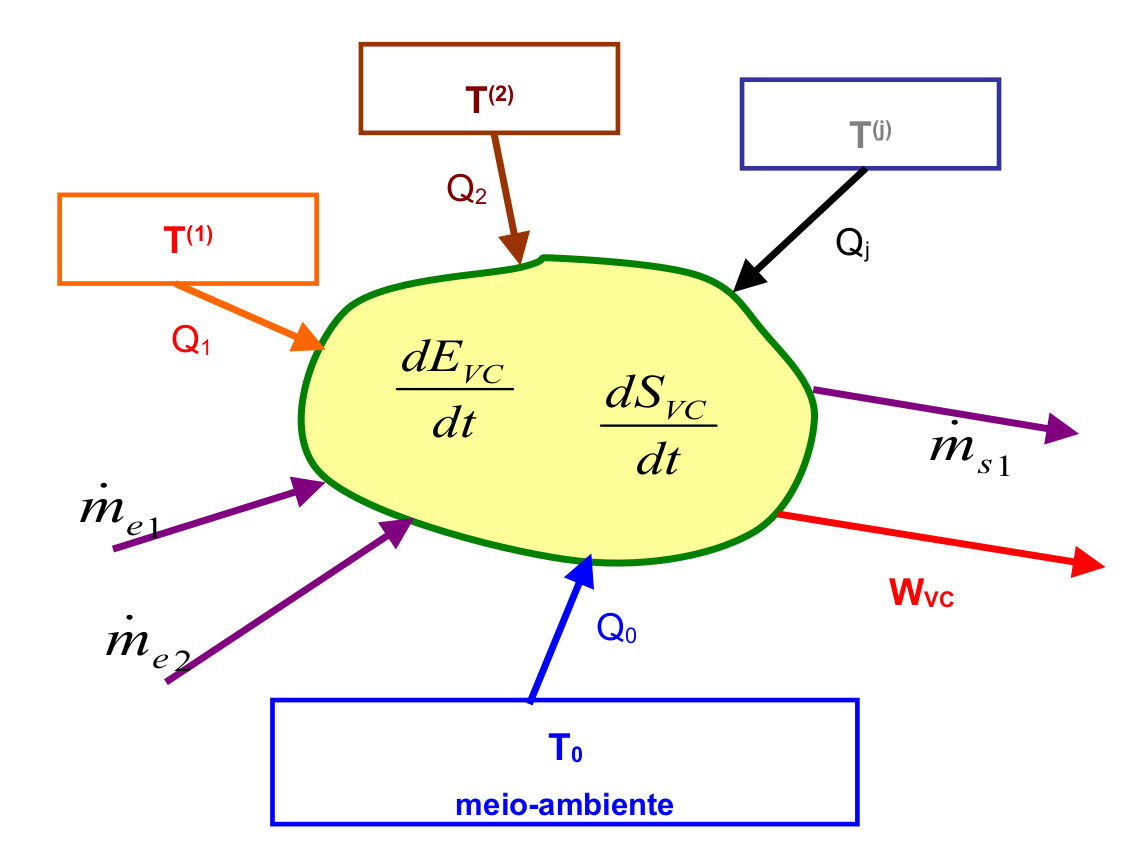
\includegraphics[
            width=\textwidth
        ]   {thermodynamicInteractionsOpenSystem.tex}

        \label{fig:thermodynamicInteractionsOpenSystem}
    \end{figure}

    Assim, a variação da energia total por unidade de tempo no interior do
    volume de controle será dada pelo balanço líquido das vazões de energia
    interna transportadas pelas vazões das massas que entram e saem do volume
    de controle, adicionadas da potência do calor que entra ou sai do volume de
    controle, e subtraídas do trabalho associado ao deslocamento da superfície
    de controle por unidade de tempo, da potência de eixo, e das potências de
    fluxo líquidas associadas às vazões das massas que entram e saem do
    volume de controle.  Matematicamente, podemos escrever, agrupando os termos
    das somatórias das massas que entram ou saem:
    %
    \begin{equation} \label{eq:2.14}
        \begin{aligned}
        \diff{\gsub{totalEnergy}{controlVolume}}
        &=
        \diff
        \left(
            \gls{mass}
            \gls{intTotalEnergy}
        \right)_{\gls{controlVolume}} \\
        &=
        \underset{\gls{inlet}}{\sum }{
            \idiff\gsub{mass}{inlet}
            \left(
                \gls{intInternalEnergy}
                +
                \gls{pressure}
                \gls{specificVolume}
                +
                \frac{\gls{velocityComp}^2}{2}
                +
                \gls{gravityComp}
                \gls{zAxis}
            \right)_{\gls{inlet}}
        }
        -
        \underset{\gls{outlet}}{\sum }{
            \idiff\gsub{mass}{outlet}
            \left(
                \gls{intInternalEnergy}
                +
                \gls{pressure}
                \gls{specificVolume}
                +
                \frac{\gls{velocityComp}^2}{2}
                +
                \gls{gravityComp}
                \gls{zAxis}
            \right)_{\gls{outlet}}
        }
        +\\
        %
        &+
        \underset{j \neq 0}{\sum }{
            \idiff\gls{heatTransfer}_j
        }
        +
        \idiff\gsub{heatTransfer}{environmentState}
        -
        \idiff\gsub{workTransfer}{controlVolume}\\
        \end{aligned}
    \end{equation}
    %
    ou, na forma de equação diferencial:
	%
	\begin{equation} \label{eq:2.15}
        \begin{aligned}
        \DDt{\gsub{totalEnergy}{controlVolume}}
        &=
        \DDt{}
        \left(
            \gls{mass}
            \gls{intTotalEnergy}
        \right)_{\gls{controlVolume}} \\
        &=
        \underset{\gls{inlet}}{\sum }{
            \gsub{massFlowRate}{inlet}
            \left(
                \gls{intInternalEnergy}
                +
                \gls{pressure}
                \gls{specificVolume}
                +
                \frac{\gls{velocityComp}^2}{2}
                +
                \gls{gravityComp}
                \gls{zAxis}
            \right)_{\gls{inlet}}
        }
        -
        \underset{\gls{outlet}}{\sum }{
            \gsub{massFlowRate}{outlet}
            \left(
                \gls{intInternalEnergy}
                +
                \gls{pressure}
                \gls{specificVolume}
                +
                \frac{\gls{velocityComp}^2}{2}
                +
                \gls{gravityComp}
                \gls{zAxis}
            \right)_{\gls{outlet}}
        }
        +\\
        %
        &+
        \underset{j \neq 0}{\sum }{
            \gls{heatTransferRate}_j
        }
        +
        \gsub{heatTransferRate}{environmentState}
        -
        \gsub{workTransferRate}{controlVolume}\,.\\
        \end{aligned}
    \end{equation}


    \section{A Propriedade Termodinâmica Entalpia}

    Vamos definir então a propriedade termodinâmica entalpia $\gls{enthalpy} =
    \gls{internalEnergy} + \gls{pressure}\gls{volume}$, bem como a entalpia
    específica $\gls{intEnthalpy} = \gls{intInternalEnergy} +
    \gls{pressure}\gls{specificVolume}$. Este importante agrupamento aparecerá
    repetidamente de agora em adiante e não apenas no contexto de volume de
    controle. De fato, como já salientamos, é uma consequência da sua definição
    que as propriedades termodinâmicas uma vez criadas se desprendam do
    contexto em que foram definidas e se agreguem ao conjunto de propriedades
    termodinâmicas, passando a ter vida própria e independente. Assim ocorrerá
    com a entalpia, propriedade extensiva, que surgiu associada aos trabalhos
    de fluxo das vazões de massa, mas existe ao interior de qualquer sistema
    termodinâmico fechado ou aberto. De fato, qualquer combinação de
    propriedades termodinâmicas poderia se qualificar por sua vez como
    propriedade termodinâmica. Então, revendo a definição de propriedades
    termodinâmicas, você saberia dizer por que o produto
    \gls{pressure}\gls{volume} é uma propriedade e o produto
    \gls{internalEnergy}\gls{volume} não pode ser?

    Agrupando-se adequadamente, a equação completa da Primeira Lei para volume
    de controle ficará:
    %
    \begin{equation} \label{eq:2.15a}
        \begin{aligned}
        \DDt{\gsub{totalEnergy}{controlVolume}}
        &=
        \DDt{}
        \left(
            \gls{mass}
            \gls{intTotalEnergy}
        \right)_{\gls{controlVolume}} \\
        &=
        \underset{\gls{inlet}}{\sum }{
            \gsub{massFlowRate}{inlet}
            \left(
                \gls{intEnthalpy}
                +
                \frac{\gls{velocityComp}^2}{2}
                +
                \gls{gravityComp}
                \gls{zAxis}
            \right)_{\gls{inlet}}
        }
        -
        \underset{\gls{outlet}}{\sum }{
            \gsub{massFlowRate}{outlet}
            \left(
                \gls{intEnthalpy}
                +
                \frac{\gls{velocityComp}^2}{2}
                +
                \gls{gravityComp}
                \gls{zAxis}
            \right)_{\gls{outlet}}
        }
        +\\
        %
        &+
        \underset{j \neq 0}{\sum }{
            \gls{heatTransferRate}_j
        }
        +
        \gsub{heatTransferRate}{environmentState}
        -
        \gsub{workTransferRate}{controlVolume}\\
        \end{aligned}
    \end{equation}
    %
    ou, na forma diferencial,
    %
    \begin{equation} \label{eq:2.16}
        \begin{aligned}
        \diff{\gsub{totalEnergy}{controlVolume}}
        &=
        \diff
        \left(
            \gls{mass}
            \gls{intTotalEnergy}
        \right)_{\gls{controlVolume}} \\
        &=
        \underset{\gls{inlet}}{\sum }{
            \idiff\gsub{mass}{inlet}
            \left(
                \gls{intEnthalpy}
                +
                \frac{\gls{velocityComp}^2}{2}
                +
                \gls{gravityComp}
                \gls{zAxis}
            \right)_{\gls{inlet}}
        }
        -
        \underset{\gls{outlet}}{\sum }{
            \idiff\gsub{mass}{outlet}
            \left(
                \gls{intEnthalpy}
                +
                \frac{\gls{velocityComp}^2}{2}
                +
                \gls{gravityComp}
                \gls{zAxis}
            \right)_{\gls{outlet}}
        }
        +\\
        %
        &+
        \underset{j \neq 0}{\sum }{
            \idiff\gls{heatTransfer}_j
        }
        +
        \idiff\gsub{heatTransfer}{environmentState}
        -
        \idiff\gsub{workTransfer}{controlVolume}\,.\\
        \end{aligned}
    \end{equation}

    Vejamos em seguida alguns casos particulares de modelos com volume de
    controle.


    \section{O Regime Permanente}

    Chamamos regime permanente aquele para o qual o tempo não tem significado,
    ou seja, desaparecem os termos explícitos no tempo e todos os demais termos
    são constantes. Podemos então escrever:
    %
    \begin{equation} \label{eq:2.17}
        0
        =
        \underset{\gls{inlet}}{\sum }{
            \gsub{massFlowRate}{inlet}
            \left(
                \gls{intEnthalpy}
                +
                \frac{\gls{velocityComp}^2}{2}
                +
                \gls{gravityComp}
                \gls{zAxis}
            \right)_{\gls{inlet}}
        }
        -
        \underset{\gls{outlet}}{\sum }{
            \gsub{massFlowRate}{outlet}
            \left(
                \gls{intEnthalpy}
                +
                \frac{\gls{velocityComp}^2}{2}
                +
                \gls{gravityComp}
                \gls{zAxis}
            \right)_{\gls{outlet}}
        }
        +
        \underset{j \neq 0}{\sum }{
            \gls{heatTransferRate}_j
        }
        +
        \gsub{heatTransferRate}{environmentState}
        -
        \gsub{workTransferRate}{controlVolume}\,.
    \end{equation}

    Se o volume de controle for adiabático e as energias cinéticas e
    potenciais puderem ser desprezadas, um caso bem comum na modelagem de
    problemas:
	%
	\begin{equation} \label{eq:2.18}
        \gsub{workTransferRate}{controlVolume}
        =
        \underset{\gls{inlet}}{\sum }{
            \gsub{massFlowRate}{inlet}
            \gsub{intEnthalpy}{inlet}
        }
        -
        \underset{\gls{outlet}}{\sum }{
            \gsub{massFlowRate}{outlet}
            \gsub{intEnthalpy}{outlet}
        }\,.
    \end{equation}

    Se não houver realização de trabalho no volume de controle, mas houver
    fluxo de calor e se as energias cinéticas e potenciais puderem ser
    desprezadas:
	%
	\begin{equation} \label{eq:2.19}
        \gsub{heatTransferRate}{controlVolume}
        =
        \underset{\gls{inlet}}{\sum }{
            \gsub{massFlowRate}{inlet}
            \gsub{intEnthalpy}{inlet}
        }
        -
        \underset{\gls{outlet}}{\sum }{
            \gsub{massFlowRate}{outlet}
            \gsub{intEnthalpy}{outlet}
        }\,.
    \end{equation}

    As \cref{eq:2.17,eq:2.18,eq:2.19} são efetivamente algébricas. Em que
    circunstâncias da vida real você imaginaria ser adequada a hipótese de
    regime permanente?


    \section{O Regime Transiente}

    Seja agora o regime não-permanente ou transiente. Devemos incluir os termos
    explícitos no tempo e, agora cuidado, todos os termos são funções do tempo.
    Então, a \cref{eq:2.16}, uma vez integrada entre os estados 1 e 2, fornece:
	%
	\begin{equation} \label{eq:2.20}
        \begin{aligned}
        \left(
            \state{\gls{mass}}{2}
            \state{\gls{intTotalEnergy}}{2}
            -
            \state{\gls{mass}}{1}
            \state{\gls{intTotalEnergy}}{1}
        \right)_{\gls{controlVolume}}
        &=
        \underset{\gls{inlet}}{\sum }{
            \int\limits_1^2{
                \left(
                    \gls{intEnthalpy}
                    +
                    \frac{\gls{velocityComp}^2}{2}
                    +
                    \gls{gravityComp}
                    \gls{zAxis}
                \right)_{\gls{inlet}}
            }\idiff\gsub{mass}{inlet}
        }
        -
        \underset{\gls{outlet}}{\sum }{
            \int\limits_1^2{
                \left(
                    \gls{intEnthalpy}
                    +
                    \frac{\gls{velocityComp}^2}{2}
                    +
                    \gls{gravityComp}
                    \gls{zAxis}
                \right)_{\gls{outlet}}
            }\idiff\gsub{mass}{outlet}
        }
        +\\
        %
        &+
        \underset{j \neq 0}{\sum }{
            \fprocess{heatTransfer}{1}{2}{j}
        }
        +
        \fprocess{heatTransfer}{1}{2\gls{environmentState}}
        -
        \fprocess{workTransfer}{1}{2}{\gls{controlVolume}}\,.\\
        \end{aligned}
    \end{equation}
    %
    \noindent na qual as integrais não poderão ser resolvidas enquanto não se
    definirem $(\gls{intEnthalpy} + \frac{\gls{velocityComp}^2}{2} +
    \gls{gravityComp}\gls{zAxis})_{\gls{inlet}}$ e $(\gls{intEnthalpy} +
    \frac{\gls{velocityComp}^2}{2} +
    \gls{gravityComp}\gls{zAxis})_{\gls{outlet}}$, bem como a história das
    massas que entram e saem do volume de controle \idiff{\gsub{mass}{inlet}}
    e \idiff{\gsub{mass}{outlet}} ao longo do processo que vai do estado 1 ao
    estado 2. Esta expressão é quase sempre utilizada conjuntamente com a
    conservação da massa:
    %
    \begin{equation} \label{eq:2.21}
        \left(
            \state{\gls{mass}}{2}
            -
            \state{\gls{mass}}{1}
        \right)_{\gls{controlVolume}}
        =
        \underset{\gls{inlet}}{\sum }{
            \int\limits_1^2{
            }\idiff\gsub{mass}{inlet}
        }
        -
        \underset{\gls{outlet}}{\sum }{
            \int\limits_1^2{
            }\idiff\gsub{mass}{outlet}
        }
        =
        \underset{\gls{inlet}}{\sum }{
            \fprocess{mass}{1}{2}{\gls{inlet}}
        }
        -
        \underset{\gls{outlet}}{\sum }{
            \fprocess{mass}{1}{2}{\gls{outlet}}
        }\,.
    \end{equation}

    Note que \fprocess{mass}{1}{2}{\gls{inlet}}  e
    \fprocess{mass}{1}{2}{\gls{outlet}} representam respectivamente toda a
    massa que entrou e toda a massa que saiu através de cada porta de entrada
    ou saída durante o processo determinado que ocorreu do estado 1 até o
    estado 2.

    Existem muitas possibilidades para processos que ocorrem em um sistema
    aberto, muitas delas em regime não permanente. Você consegue imaginar um
    problema real e modelá-lo utilizando a expressão para a Primeira Lei?
